% ============================================================
% CIC 2026 submission -- Springer LNCS template
% Compile: latexmk -pdf main.tex   (requires llncs.cls, see README)
%
% This paper is deliberately DISJOINT from the CoRL 2026 TaCo
% submission: TaCo claims the discrete gesture command channel
% (vocabulary, classification, HRI user study); this paper claims
% the learned CONTINUOUS velocity policy, the imitation pipeline,
% and the perturbation-robustness methodology and results.
% ============================================================
\documentclass[runningheads]{llncs}

\usepackage{amsmath}
\usepackage{amssymb}
\usepackage{graphicx}
\usepackage{booktabs}
\usepackage{xcolor}

% Placeholder marker: everything highlighted like this needs your input.
\newcommand{\placeholder}[1]{\textcolor{red}{[\textbf{PLACEHOLDER:} #1]}}

\begin{document}

\title{From Hand-Crafted Rules to Learned Policies: Robust Continuous
Finger-Motion Guidance of a Collaborative Robot through a Capacitive
Tactile Skin}
\titlerunning{Learned Continuous Tactile Guidance}

% ------------------------------------------------------------------
\author{\placeholder{Author One}\inst{1}\orcidID{0000-0000-0000-0000} \and
\placeholder{Author Two}\inst{1} \and
\placeholder{Author Three}\inst{2}}
\authorrunning{\placeholder{A. One} et al.}
\institute{\placeholder{Institution One, City, Country}
\email{\placeholder{one@example.edu}}
\and
\placeholder{Institution Two, City, Country}}
% ------------------------------------------------------------------

\maketitle

\begin{abstract}
Capacitive tactile skins let an operator guide a collaborative robot by
sliding a finger over the robot body, but the controllers that translate
touch into motion are almost always hand-crafted: a pipeline of centroid
tracking, thresholds, and mode heuristics whose dozens of tuned parameters
are brittle against sensor drift, damaged cells, and gain variation.
We present a learned alternative and, equally importantly, a way to
\emph{prove} that it is more robust.
First, we record the rule-based controller as a teacher and train a
lightweight spatiotemporal policy---a location-preserving convolutional
encoder with per-channel soft-argmax keypoints, followed by a recurrent
temporal head---that maps raw $10\times10$ capacitance sequences directly
to 6-DOF end-effector velocity commands and interaction modes.
A geometry-aware augmentation scheme (touch-pattern flips and translations
with consistently transformed velocity targets) multiplies the effective
coverage of a five-minute demonstration corpus.
Second, we introduce a \emph{faithful-replay robustness benchmark}: recorded
episodes are re-played through the unmodified deployed implementations of
both the rule pipeline and the learned policy while calibrated perturbations
---baseline drift, dead taxels, gain error, and Gaussian noise---are
injected into the capacitance stream, and both are scored against the
clean-input teacher command.
The learned policy matches the teacher on clean input
(1.45\,cm/s velocity RMSE, 92.6\% mode accuracy) and degrades far more
gracefully than the rules under drift, dead taxels (up to 20\% of the
array), and gain error, while a targeted noise experiment exposes an honest
failure mode of temporal-difference input channels.
The policy runs in 1.9\,ms per inference on a desktop CPU with 0.23\,M
parameters, well within a 60\,Hz control budget.
\keywords{Tactile sensing \and Imitation learning \and Human--robot
interaction \and Robustness evaluation \and Capacitive skin}
\end{abstract}

% ==================================================================
\section{Introduction}
\label{sec:intro}

A tactile skin wrapped around a robot link invites the most direct form of
robot guidance imaginable: place a finger on the robot and slide it in the
direction the tool should move.  Systems that realize this interaction
today do so with hand-crafted signal-processing pipelines.  A touch
centroid is extracted from the thresholded capacitance image, its
frame-to-frame displacement is scaled into a velocity command, and a stack
of auxiliary heuristics---pressure thresholds for push and pull modes,
hold counters, hysteresis bands, grace periods---arbitrates between
interaction modes.  Such controllers work, and they work well enough to
serve as a product feature.  But they inherit the classic weaknesses of
rule-based perception.  Every threshold is tuned to one sensor, one
mounting, one operator, and one day's baseline; capacitive arrays drift
with temperature and humidity, individual taxels die, and gain varies
across fabrication batches.  Each new robustness patch adds parameters
that interact with the existing ones.

This paper asks whether a \emph{learned} policy can replace the rule
pipeline for continuous tactile guidance, and---the question that is
usually left unanswered---how to demonstrate that the replacement is more
than a costly imitation.  Our answer has two parts.

\textbf{An imitation pipeline that inherits the rules' competence.}
We treat the deployed rule-based controller as a teacher.  While an
operator interacts with the skin, we record synchronized capacitance
frames together with the teacher's velocity command and mode decision,
yielding labeled episodes without any manual annotation.  A compact
CNN--GRU policy is trained offline on these episodes.  Its convolutional
encoder deliberately avoids global average pooling: a per-channel
soft-argmax (spatial softmax) layer preserves \emph{where} each learned
feature fires on the taxel grid, which is precisely the information that
determines the commanded direction.  A geometry-aware augmentation scheme
exploits the physical symmetries of the sensor: touch patterns are flipped
and translated on the grid while the velocity targets and hand-crafted
auxiliary features are transformed consistently, multiplying a
five-minute demonstration corpus by an order of magnitude.

\textbf{A robustness benchmark that both pipelines take identically.}
Offline agreement with the teacher cannot show superiority over the
teacher---by construction, perfect agreement only ties the rules.  We
therefore built a \emph{faithful-replay benchmark}: recorded episodes are
streamed through the \emph{unmodified deployed implementations} of both
controllers (including all stateful counters, smoothing filters, and
confidence gates) while calibrated sensor perturbations are injected into
the capacitance stream.  Both controllers are scored against the
clean-input teacher command at every frame.  The benchmark validates its
own fidelity: with zero perturbation, the replayed rule pipeline
reproduces the recorded teacher command exactly on 89.8--97.3\% of frames,
with residual deviations confined to episode-boundary counter states.

On this benchmark the learned policy is not merely equal to its teacher.
Under baseline drift it holds a 30--40\% lower velocity error than the
rules until both collapse at extreme drift; with 20\% of taxels dead its
error rises by only 32\% while remaining $1.7\times$ below the rules; and
it is more tolerant to gain error on both sides of unity.  A targeted
noise sweep also exposes a genuine weakness---temporal-difference input
channels amplify uncorrelated per-frame noise---which we analyze and
discuss rather than hide.

Contributions:
\begin{enumerate}
  \item An end-to-end imitation pipeline that converts a deployed
  rule-based tactile guidance controller into training supervision for a
  continuous velocity policy, requiring no manual labeling.
  \item A location-preserving policy architecture (spatial-softmax
  convolutional encoder + recurrent temporal head, 0.23\,M parameters,
  1.9\,ms CPU inference) and a geometry-aware augmentation scheme that
  transforms tactile frames, auxiliary features, and velocity targets
  consistently.
  \item A faithful-replay robustness benchmark for tactile interfaces,
  with four calibrated perturbation families, that scores the deployed
  implementations of rule-based and learned controllers under identical
  corruptions---and results showing the learned policy degrades more
  gracefully on three of the four families.
\end{enumerate}

% ==================================================================
\section{Related Work}
\label{sec:related}

\subsubsection{Tactile skins for physical human--robot interaction.}
Large-area robot skins have progressed from rigid pressure pads to
conformal capacitive, resistive, and multimodal arrays
\cite{dahiya2010tactile,cannata2008embedded,mittendorfer2011humanoid},
including textile and fabric-based sensors that wrap curved robot links
\cite{robosweater,luo2021conformal,tamura2020woven}.  Most systems use the
skin for safety (collision detection, contact localization) or for
perception during manipulation \cite{yuan2017gelsight,luo2025tactileroboticsoutlook}.
A smaller body of work uses skin contact as an \emph{input channel}:
touch-gesture classification on robot surfaces
\cite{liu2022machine,fitter2016qualitative} and continuous lead-through
control via force/torque interpretation \cite{Iskandar2024ScienceRobotics}.
Continuous \emph{velocity} guidance from a taxel array is typically
realized with hand-crafted centroid-tracking controllers; we are not aware
of prior work that both learns this mapping end-to-end from the raw taxel
stream and quantifies its robustness against the rule-based controller it
replaces.

\subsubsection{Learning from demonstration and behavior cloning.}
Casting controller construction as supervised imitation is a long-standing
idea \cite{pomerleau1989alvinn,argall2009survey}.  Our setting is unusual
in that the demonstrator is itself a \emph{program}, which sidesteps the
multimodality that plagues human demonstrations \cite{ross2011dagger} and
makes plain regression well-posed, but bounds the achievable policy by the
teacher's competence on clean input.  The value of learning then lies in
generalization under input corruption---exactly what our benchmark
measures.  Related programmatic-teacher setups appear in autonomous
driving \cite{chen2020learning} and locomotion \cite{lee2020learning},
where privileged or scripted experts supervise sensor-space students.
Spatial-softmax feature points originate in end-to-end visuomotor policy
learning \cite{levine2016end,finn2016deep}; we show they matter even on a
$10\times10$ tactile grid, where global pooling destroys the location
information that determines command direction.

\subsubsection{Robustness evaluation of tactile pipelines.}
Sensor-corruption benchmarks are standard in vision
\cite{hendrycks2019robustness} but rare in tactile control, where
evaluations usually report accuracy on clean held-out data.  Perturbation
studies exist for tactile object recognition \cite{taunyazov2019tactile},
yet controller-level comparisons under identical corruption are missing.
Our replay harness is closest in spirit to log-replay evaluation in
autonomous driving \cite{caesar2020nuscenes}, transplanted to the tactile
interface setting with perturbation models specific to capacitive arrays
(baseline drift, dead taxels, gain error, thermal noise).

% ==================================================================
\section{System Overview}
\label{sec:system}

\subsection{Sensing Substrate and Control Loop}

Our testbed is a capacitive tactile skin providing a $10\times10$ grid of
taxels mounted on the end link of a 6-DOF collaborative arm (TM5-900).
The skin outputs, per frame, a matrix of relative capacitance changes
(percentage deviation from a per-session calibration baseline); touching
the surface produces negative deviations roughly proportional to contact
pressure.  A three-frame moving average is computed on-device alongside
the instantaneous signal.  Frames are consumed by the controller at
approximately 60\,Hz.
\placeholder{One to two sentences on skin construction and readout
electronics, with a citation to your hardware publication if available.
Kept intentionally brief here: the hardware is not a contribution of this
paper.}

\subsection{The Rule-Based Teacher}
\label{sec:teacher}

The deployed controller---our teacher and our baseline---follows the
canonical centroid-tracking design.  Taxels below a touch threshold
$\tau=-3.0$ are clustered by connected components; a pressure-weighted
centroid $(r_t, c_t)$ is tracked with hysteresis.  The normalized centroid
displacement $(\Delta r_t, \Delta c_t)$, after a deadband and gain, is
mapped to end-effector velocity: column motion commands $v_x$, row motion
commands $v_z$.  Two pressure-gated modes overlay this mapping: a hard
press (peak below a push threshold, displacement within a hold deadband
for $k$ consecutive frames) commands a \emph{push} along $+v_y$, and a
two-finger pinch commands a \emph{pull} along $-v_y$, both with
pressure-modulated speed.  Release logic, grace periods, and axis locks
complete the pipeline.  In total the controller exposes roughly thirty
tuned parameters.  This is a competent, production-quality design---and
every one of its thresholds silently assumes a clean, calibrated,
undamaged sensor.

\subsection{Teacher-Supervised Data Collection}

During recording sessions an operator interacts freely with the skin while
the teacher runs.  At each control tick we store the instantaneous and
averaged capacitance matrices, the teacher's 6-DOF velocity command
$\mathbf{v}_t^\ast \in \mathbb{R}^6$, its mode decision
$m_t^\ast \in \{\textit{stop}, \textit{move}, \textit{push},
\textit{pull}\}$, and the hand-crafted intermediate features (centroid,
displacement, speed, peak and mean pressure, touch presence).  The corpus
used in this paper comprises \textbf{8 episodes, 18{,}551 frames
($\approx$5.2 minutes)} across two sessions: free omnidirectional swiping,
and a push/pull-focused session.  No frame was manually labeled.
Rotational axes were not exercised and are locked to zero throughout.

% ==================================================================
\section{Learned Policy}
\label{sec:method}

\subsection{Input Representation}

The policy consumes a sliding window of $T{=}16$ frames.  Each frame is a
4-channel $10\times10$ image: the instantaneous capacitance deviation, its
3-frame moving average, the temporal difference between consecutive
instantaneous frames, and a binary touch mask obtained by thresholding the
averaged channel at $\tau$.  Alongside the frames, an 11-dimensional
auxiliary vector carries the teacher pipeline's own intermediate features
(normalized centroid position, raw and normalized displacement, speed,
peak and mean active pressure, touch presence, and control-frame index).
Feeding the teacher's features to the student is deliberate: it gives the
policy a warm start on the quantities the rules found useful, while the
raw frames let it learn what the rules discard.

\subsection{Location-Preserving Spatiotemporal Architecture}

\begin{figure}[t]
\centering
\fbox{\parbox[c][4.2cm][c]{0.92\textwidth}{\centering
\placeholder{Architecture diagram: 4-channel $10\times10$ frame window
$\rightarrow$ conv stem (3 layers, no pooling) $\rightarrow$ per-channel
spatial softmax keypoints + mean intensities $\rightarrow$ fusion with
auxiliary-feature MLP $\rightarrow$ GRU (128) $\rightarrow$ velocity head
(6-DOF) + mode head (4-way). Redraw in the style of your group's figures.}}}
\caption{Policy architecture. A location-preserving convolutional encoder
turns each tactile frame into soft-argmax keypoints and intensities; a
recurrent head integrates the 16-frame window and emits a 6-DOF velocity
command and an interaction mode.}
\label{fig:arch}
\end{figure}

\emph{Frame encoder.}  Three $3\times3$ convolutions (32, 64, 64 channels,
batch normalization, GELU) process each frame at full $10\times10$
resolution---no spatial pooling at any depth.  A per-channel
\emph{spatial softmax} then reduces each of the 64 feature maps
$F_k \in \mathbb{R}^{10\times10}$ to its expected image coordinate,
\begin{equation}
\mathbf{p}_k = \sum_{(i,j)} \operatorname{softmax}\!\big(F_k/\theta\big)_{ij}
\, (u_i, u_j), \qquad u \in [-1, 1],
\label{eq:ssoftmax}
\end{equation}
with a learned temperature $\theta$.  Concatenating the 64 keypoints with
the 64 per-channel mean intensities yields a 192-dimensional descriptor
that preserves \emph{where} the contact is and \emph{how hard} it presses.
The alternative---global average pooling, common in compact tactile
encoders---collapses location entirely; on a guidance task where direction
is decoded from position change, this is the single most damaging design
choice available, and we quantify its cost in
Sect.~\ref{sec:results-robust}.

\emph{Temporal head and outputs.}  Frame descriptors are fused with an
MLP-encoded auxiliary vector and passed through a single-layer GRU (128
units).  Two heads read the final hidden state: a velocity head regressing
the normalized 6-DOF command, and a 4-way mode classifier.  The full model
has \textbf{234{,}955 parameters} and runs in \textbf{1.9\,ms} per window
on a desktop CPU---an order of magnitude inside the 16\,ms control budget,
leaving headroom for embedded deployment.

\subsection{Geometry-Aware Augmentation}
\label{sec:augment}

Five minutes of demonstration cannot cover the product space of contact
locations, directions, and pressures.  The sensor's geometry, however,
provides exact symmetries.  During training each sampled window is, with
probability $0.5$ per axis, \emph{flipped} on the taxel grid---and the
transformation is propagated consistently through every affected quantity:
a column flip negates $v_x$ (and the $r_z$ target, if present), mirrors
the centroid column, and negates the column displacement features; a row
flip acts analogously on $v_z$, $r_x$, and the row features.  Windows are
additionally \emph{translated} by up to $\pm2$ taxels, bounded such that
no active cell leaves the grid (targets unchanged, centroid features
shifted), and perturbed with Gaussian noise scaled to a fraction of each
channel's training standard deviation.  The flip group alone multiplies
directional coverage by four; translation decouples the learned mapping
from absolute contact position.  Mode labels are invariant under all three
transforms.  Augmentation is applied only to training windows, never to
validation data.

\subsection{Training Protocol}

Windows are split by \emph{episode} (never within an episode): 6 training
episodes yield 13{,}847 windows, 2 held-out episodes (one per session)
yield 4{,}584 validation windows.  Normalization statistics use training
data only.  The loss is a weighted sum of a Smooth-$L_1$ velocity term and
a class-balanced cross-entropy mode term ($\lambda_{\text{mode}}=0.2$),
with per-sample weights that de-emphasize \emph{stop} frames and emphasize
the rarer \emph{pull} class.  We train with AdamW (learning rate $10^{-3}$,
weight decay $10^{-4}$, batch 128), plateau-based decay, and early
stopping; the reported model converged at epoch~6.  Rotational output
axes are constrained to zero, matching the recorded task space.

% ==================================================================
\section{Faithful-Replay Robustness Benchmark}
\label{sec:benchmark}

\subsection{Design}

The benchmark answers one question: \emph{when the sensor misbehaves, which
controller keeps translating operator intent correctly?}  Three design
decisions distinguish it from standard offline evaluation.

\emph{(1) Deployed implementations, not re-implementations.}
Both controllers are exercised through their unmodified runtime classes.
Recorded episodes are streamed frame-by-frame into a sensor emulation
layer; the rule pipeline runs with all its stateful machinery (hold
counters, hysteresis, grace periods, smoothing), and the learned policy
runs with its deployed buffering, normalization, and confidence gating.
Nothing is idealized.

\emph{(2) Ground truth from clean input.}
The reference at frame $t$ is the teacher command recorded on the
\emph{clean} sensor stream.  Both controllers then receive an identically
\emph{perturbed} stream.  A controller scores well if corruption does not
change what it believes the operator wants---the operator's finger, after
all, is doing the same thing regardless of sensor health.

\emph{(3) Self-validation.}
At zero perturbation the replayed rule pipeline must reproduce its own
recorded output.  It does: 89.8\% and 97.3\% of frames match exactly on
the two held-out episodes, with residuals traceable to stateful-counter
initial conditions at episode boundaries.  This closes the loop on harness
fidelity before any perturbation is trusted.

\subsection{Perturbation Families}

Four families model the dominant failure modes of capacitive arrays.
All are injected consistently into both the instantaneous and the
moving-average channel (noise is correctly attenuated in the average, as
the physical sensor stack would).
\textbf{Baseline drift}: a uniform offset toward the touch threshold,
modeling thermal/humidity drift between calibrations
(0--3.0 units; the touch threshold is $-3.0$).
\textbf{Dead taxels}: a random fraction of cells clamped to zero
(0--20\%), modeling broken electrodes.
\textbf{Gain error}: multiplicative scaling (0.5--1.3$\times$), modeling
batch variation and mounting differences.
\textbf{Gaussian noise}: i.i.d.\ per-cell noise
($\sigma \in [0, 4]$ units), modeling electromagnetic interference.
Velocity error is reported as linear-axis RMSE against the clean-input
teacher command; mode agreement as the fraction of frames whose canonical
mode (\textit{stop}/\textit{move}/\textit{push}/\textit{pull}) matches.

% ==================================================================
\section{Results}
\label{sec:results}

\subsection{Offline Imitation Fidelity}

\begin{figure}[t]
\centering
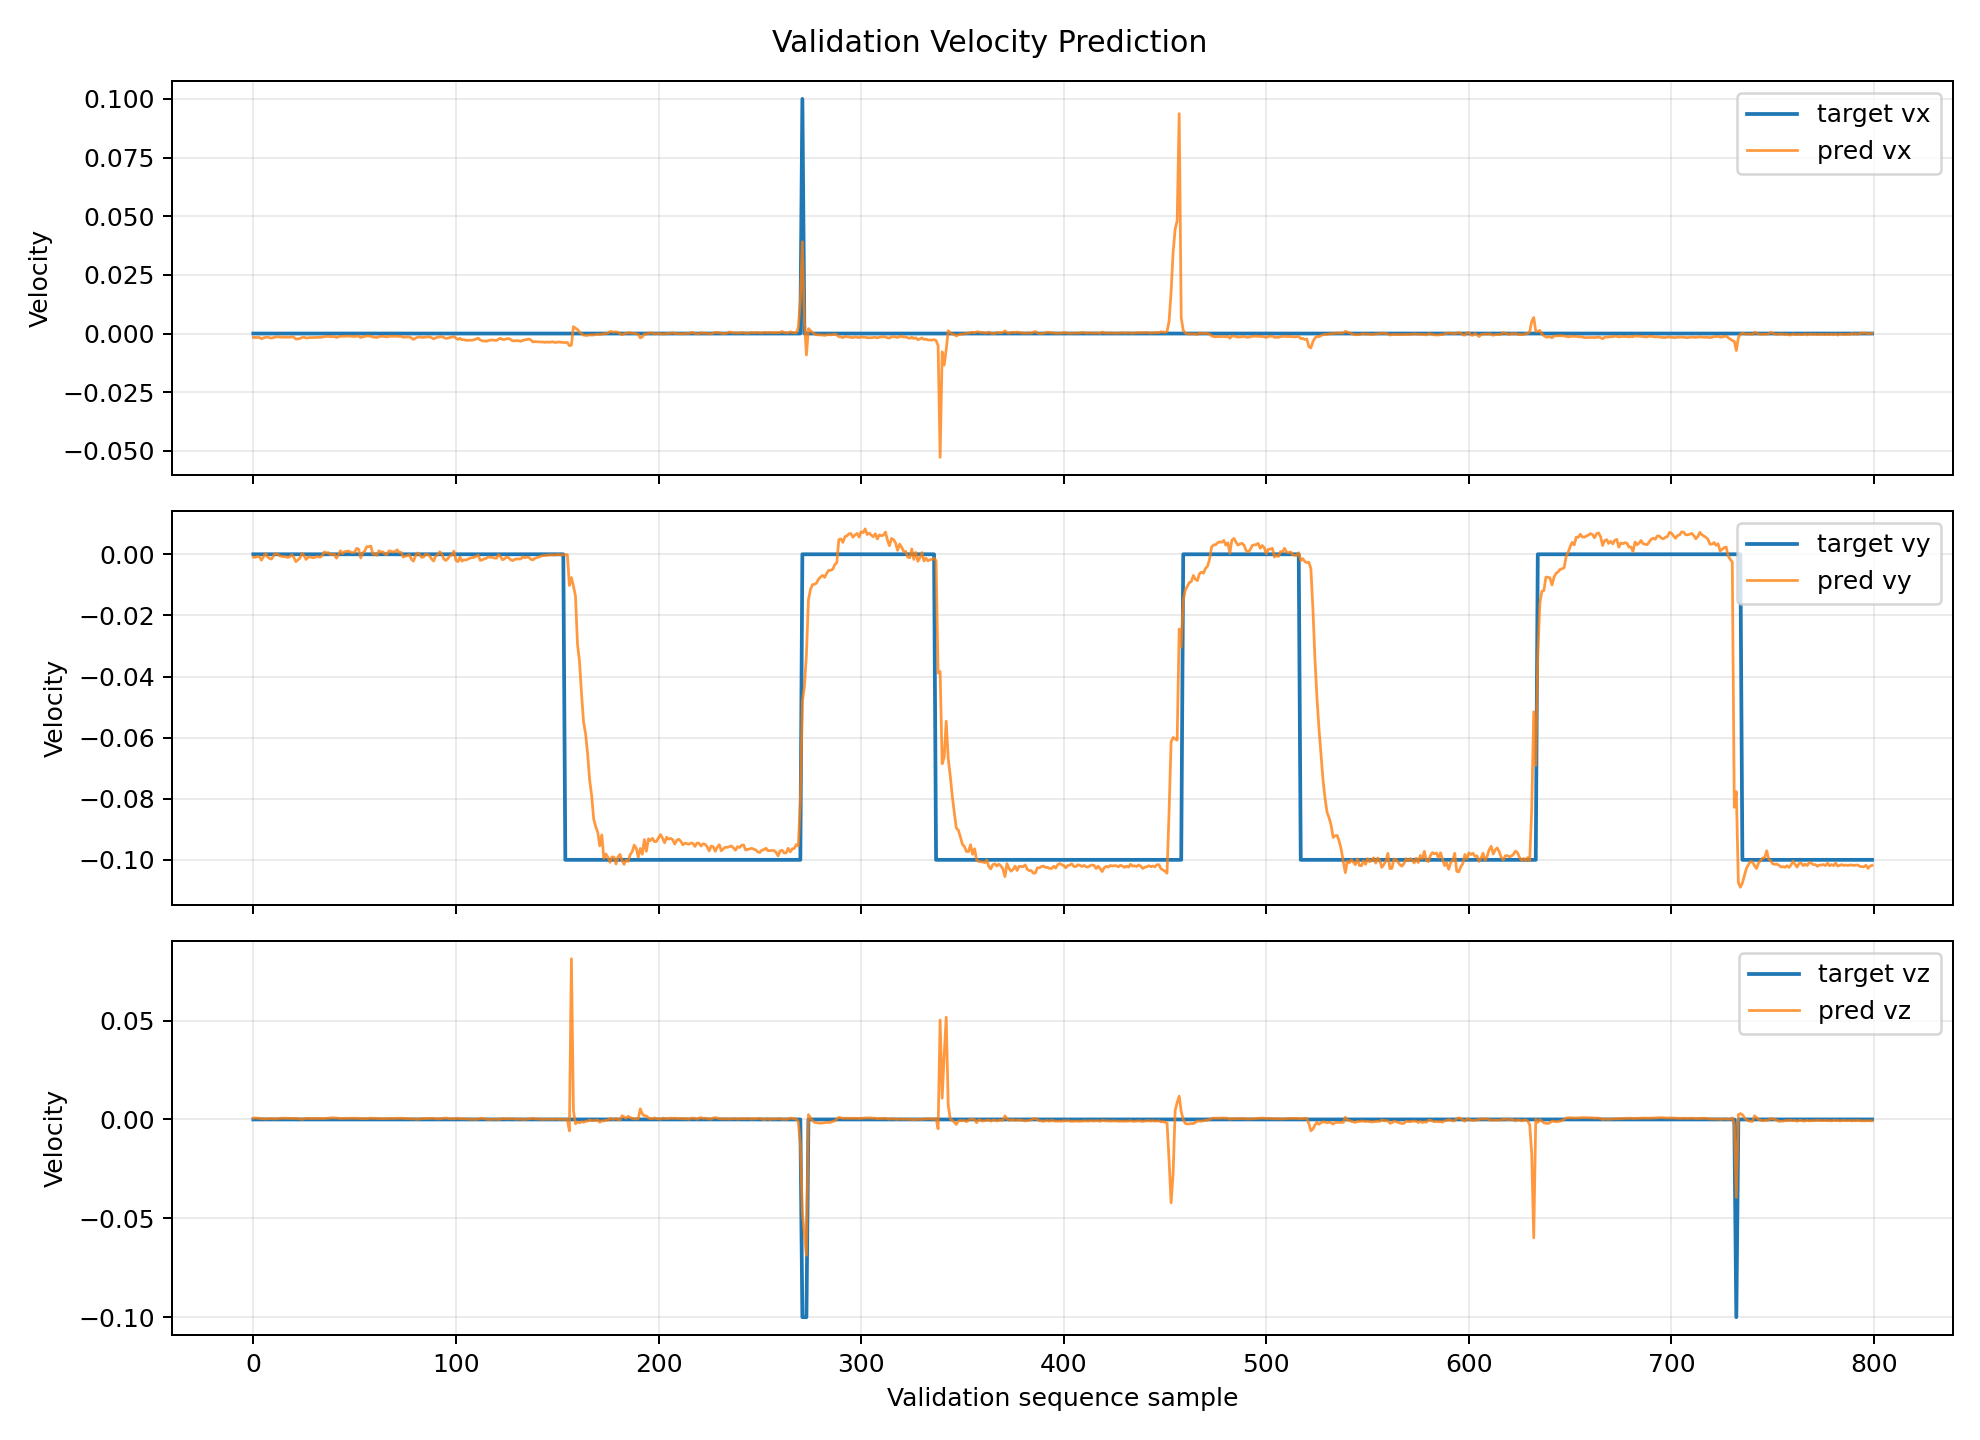
\includegraphics[width=0.85\textwidth]{figure/validation_velocity_timeseries.png}
\caption{Predicted vs.\ teacher velocity on held-out validation episodes
(first 800 windows; $v_x$, $v_y$, $v_z$ from top to bottom). The policy
reproduces direction changes, push/pull events ($v_y$), and stop phases.}
\label{fig:timeseries}
\end{figure}

On the two held-out episodes the policy attains a linear-velocity RMSE of
\textbf{1.45\,cm/s} against teacher commands whose magnitudes reach
10\,cm/s (per-axis $R^2$: 0.82 / 0.83 / 0.81 for $v_x/v_y/v_z$), and
\textbf{92.6\%} mode accuracy.  Mode confusions concentrate where the
teacher itself is ambiguous---\textit{stop} frames bordering
\textit{push} onsets (Fig.~\ref{fig:timeseries}).  Note that these numbers
measure agreement with the teacher; they establish that imitation
succeeded, not that the policy is better.  That question is answered next.

\subsection{Robustness under Sensor Perturbation}
\label{sec:results-robust}

\begin{table}[t]
\centering
\caption{Faithful-replay benchmark on held-out episodes (4{,}614 frames):
velocity RMSE (m/s, lower is better) and canonical-mode agreement
(higher is better) against the clean-input teacher command. Both
controllers receive identical perturbed streams. Bold marks the better
controller per condition.}
\label{tab:robust}
\begin{tabular}{llcccc}
\toprule
& & \multicolumn{2}{c}{RMSE (m/s)} & \multicolumn{2}{c}{Mode agree.} \\
\cmidrule(lr){3-4}\cmidrule(lr){5-6}
Perturbation & Level & Rules & Learned & Rules & Learned \\
\midrule
None (clean)     & --      & 0.032 & \textbf{0.014} & 0.68 & \textbf{0.93} \\
\midrule
Baseline drift   & 1.0     & 0.032 & \textbf{0.020} & 0.69 & \textbf{0.90} \\
                 & 2.0     & 0.033 & \textbf{0.024} & 0.71 & \textbf{0.84} \\
                 & 3.0     & \textbf{0.052} & 0.062 & \textbf{0.48} & 0.07 \\
\midrule
Dead taxels      & 10\%    & 0.032 & \textbf{0.015} & 0.68 & \textbf{0.93} \\
                 & 20\%    & 0.033 & \textbf{0.019} & 0.67 & \textbf{0.88} \\
\midrule
Gain error       & 0.7$\times$ & 0.036 & \textbf{0.019} & 0.61 & \textbf{0.90} \\
                 & 1.3$\times$ & 0.029 & \textbf{0.016} & 0.75 & \textbf{0.92} \\
\midrule
Gaussian noise   & $\sigma{=}0.5$ & \textbf{0.034} & 0.043 & \textbf{0.67} & 0.62 \\
                 & $\sigma{=}2.0$ & \textbf{0.041} & 0.056 & \textbf{0.56} & 0.37 \\
\bottomrule
\end{tabular}
\end{table}

\begin{figure}[t]
\centering
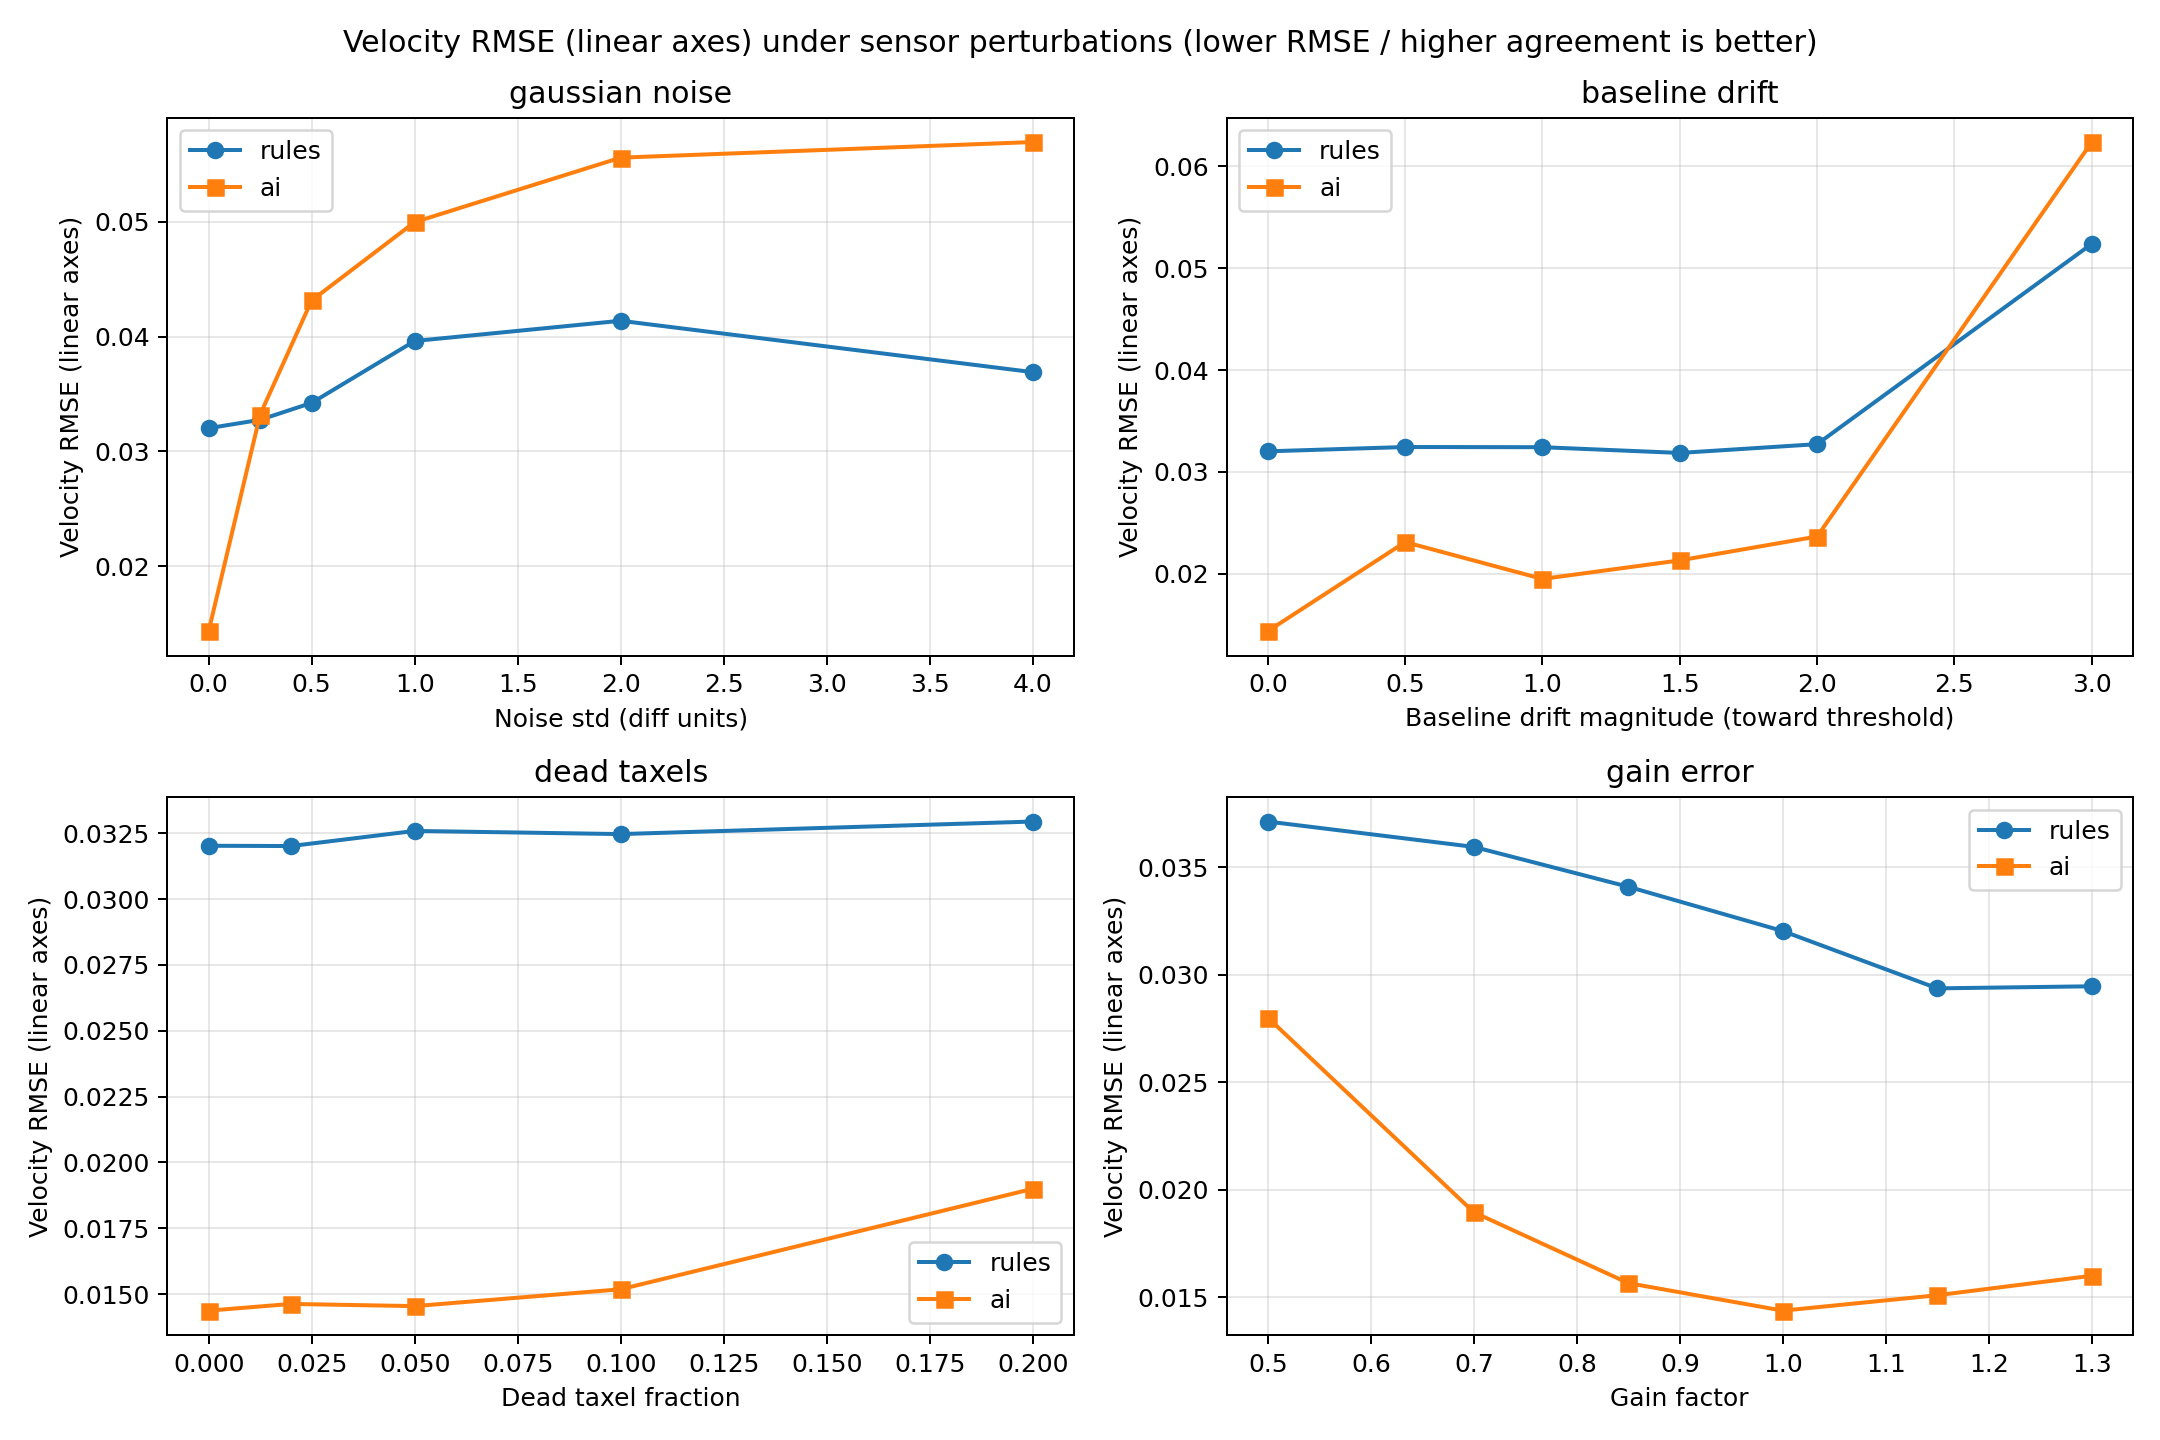
\includegraphics[width=\textwidth]{figure/rmse_vs_perturbation.png}
\caption{Velocity RMSE against the clean-input teacher command as a
function of perturbation magnitude, for the rule pipeline (circles) and
the learned policy (squares), across all four perturbation families.}
\label{fig:robust}
\end{figure}

Table~\ref{tab:robust} and Fig.~\ref{fig:robust} report the benchmark.
Three findings stand out.

\emph{The learned policy wins three of four families.}
Under baseline drift up to 2.0 units---two-thirds of the way to the touch
threshold---the policy's error stays 27--38\% below the rules', and its
mode agreement stays above 0.84 while the rules never exceed 0.71.  With
one in five taxels dead, the policy's error rises only from 0.014 to
0.019\,m/s; the convolutional encoder interpolates around missing cells,
whereas the rules' pressure-weighted centroid has no such mechanism.
Under gain error the same picture holds on both sides of unity.

\emph{Both collapse at extreme drift, for the same reason.}
At drift 3.0 the offset equals the touch threshold: every idle cell
registers as touched, touch segmentation fails, and neither controller
receives a meaningful contact signal.  This is a sensing failure, not a
control failure, and marks the boundary beyond which recalibration---not
robustness---is the remedy.

\emph{Uncorrelated noise is an honest weakness of the learned policy.}
Already at $\sigma{=}0.5$ the policy falls behind the rules.  The cause is
architectural: one input channel is a \emph{temporal difference} of
consecutive frames, which doubles the variance of i.i.d.\ noise, and the
binary touch-mask channel flickers when cell values straddle the
threshold.  The rules are partially shielded because they read only the
3-frame moving average.  The failure mode is thus attributable to input
design rather than to learning per se---and it is addressable: training
with realistic (temporally correlated) noise models, or low-pass filtering
the instantaneous channel at deployment, are direct remedies that we
discuss in Sect.~\ref{sec:limitations}.

\emph{A note on the clean-input mode gap.}
The rules' modest clean-input mode agreement (0.68) is not an error of the
replay: on a subset of recorded frames the ground-truth command reflects
manually specified teaching intent that overrides the raw rule output, and
the learned policy---trained on the intended command---captures this
intent where the raw rules diverge from it.  The learned policy thus
imitates what the operator \emph{meant}, not merely what the pipeline
\emph{did}.

\subsection{Ablation: Location-Preserving Encoding and Augmentation}

\begin{table}[t]
\centering
\caption{Effect of the location-preserving encoder and geometry-aware
augmentation on noise robustness (velocity RMSE, m/s). The baseline
variant uses a global-average-pooling encoder without geometric
augmentation. Both variants are benchmarked identically.
\placeholder{Re-run as a controlled single-variable ablation (same
sequence length and training budget) before camera-ready; current numbers
compare deployed variants that also differ in window length (8 vs.\ 16).}}
\label{tab:ablation}
\begin{tabular}{lcccc}
\toprule
Variant & Clean & Noise $\sigma{=}0.25$ & Noise $\sigma{=}0.5$ & Dead 20\% \\
\midrule
GAP encoder, no geom.\ aug. & 0.014 & 0.055 & 0.059 & 0.022 \\
Spatial softmax + geom.\ aug.\ (ours) & 0.014 & \textbf{0.033} & \textbf{0.043} & \textbf{0.019} \\
\bottomrule
\end{tabular}
\end{table}

Table~\ref{tab:ablation} compares the proposed configuration against a
variant with a global-average-pooling encoder and no geometric
augmentation.  Clean-input fidelity is identical---on in-distribution
data, either encoder suffices---but under perturbation the difference is
large: at $\sigma{=}0.25$ noise the proposed configuration's error is 40\%
lower.  Robustness, not clean accuracy, is where the architectural and
augmentation choices pay off; evaluations that report only clean held-out
metrics would miss this entirely.

% ==================================================================
\section{Limitations and Future Work}
\label{sec:limitations}

\emph{The teacher bounds the policy on clean input.}
Behavior cloning from a programmatic teacher cannot exceed the teacher
where the teacher is right; our claim is superiority under corruption, not
on clean data.  Surpassing the teacher outright requires richer
supervision---human teleoperation corrections or task-level objectives---
which our recording infrastructure supports but this paper does not
evaluate.

\emph{Noise robustness is unfinished.}
The temporal-difference channel should be trained under temporally
correlated noise models fitted to the physical sensor, and the binary
touch mask replaced by a soft (sigmoid) mask.  Both are drop-in changes to
the training pipeline.

\emph{Closed-loop evaluation.}
All results are open-loop replay: the policy's commands do not feed back
into the operator's behavior.
\placeholder{Closed-loop user study: $N$ participants guide the robot
through reach/track tasks under (a) rule pipeline, (b) learned policy,
on a healthy sensor and on a sensor with masked-off taxel regions;
report completion time and path error. This is the strongest addition
you can make before camera-ready.}

\emph{Scope.}
Rotational axes were locked to zero throughout; extending the corpus with
two-finger rotation gestures is mechanical.  Results come from a single
sensor unit and a small number of operators;
\placeholder{multi-user, multi-unit generalization data if available}.

% ==================================================================
\section{Conclusion}
\label{sec:conclusion}

We showed that the hand-crafted rule pipelines conventionally used for
continuous tactile robot guidance can be distilled into a compact learned
policy---and, through a faithful-replay benchmark that exercises the
deployed implementations of both controllers under identical calibrated
corruptions, that the learned policy is the more robust of the two under
baseline drift, dead taxels, and gain error, the failure modes that
dominate capacitive skins in practice.  The methodology is the more
transferable half of the contribution: any tactile interface with a
recorded teacher, rule-based or human, can be evaluated the same way.
The learned policy's noise weakness, traced to a temporal-difference input
channel, illustrates precisely why such benchmarks should accompany every
learned replacement of a working classical controller: on clean held-out
data the two were indistinguishable, and only under perturbation did their
differences---in both directions---become visible.

% ==================================================================
\subsubsection{Acknowledgements.}
\placeholder{Funding sources and acknowledgements.}

\subsubsection{Disclosure of Interests.}
\placeholder{The authors have no competing interests to declare that are
relevant to the content of this article. (Adjust as required.)}

% ------------------------------------------------------------------
\bibliographystyle{splncs04}
\bibliography{references}

\end{document}
